\chapter{Subspaces, Projection Operators, and Measurement as Entanglement}

Bell's theorem has left two questions on the table. What remains of entanglement when one member of a pair is disturbed, absorbed, or measured? And what, precisely, turns an ordinary interaction into a measurement? The route to an answer runs through elementary linear algebra. Properties are subspaces, probabilities are expectation values of projectors, and a measuring apparatus is another quantum system with which the object becomes entangled.

\section{Opening Motivation: Entanglement, Locality, and Measurement}

Suppose a singlet has been separated into two distant parts and one part is measured. Must quantum field theory describe a virtual exchange between them? Nothing detectable happens at the far side, and no usable message arrives there. One may rotate one spin locally with a magnetic field, changing the detailed form of the joint state, while the amount of entanglement remains fixed under that local operation. Quantitative measures of entanglement will come later; the immediate point is that two systems which no longer interact cannot change their shared entanglement merely through an operation confined to one side.

\begin{classroomqa}
\lecturetimestamp{00:00:22}
\audiencequestion{Does a measurement on one member of a spacelike-separated singlet require some virtual exchange with the other?}
\lecturerresponse{No detectable exchange occurs at the other side. A local operation may rotate one factor and alter the form in which the joint state is written, but it cannot by itself send a message or change the entanglement shared across the separation.}
\end{classroomqa}

That forces a broader notion of what counts as the partner. If one member of an entangled pair falls into a black hole, the other does not cease to be entangled; it becomes entangled with the black-hole degrees of freedom and, after evaporation, with the emitted radiation. The same idea needs no black hole. Drop one member of an entangled pair into a bathtub and let it mix violently with the water. Its individual identity may be lost in the many-body state, yet the distant particle remains entangled with the bathtub as a whole and eventually with the escaping vapor.

This is not only a story about persistence. It is also a story about reversibility. If interaction can create entanglement, then interaction can, in principle, undo it. Disentanglement is possible, but only when the systems come back into contact and interact again. Anything that can happen one way can happen the other way.

\begin{classroomqa}
\lecturetimestamp{00:04:45}
\audiencequestion{If both spins of an entangled pair are measured, do the electrons remain entangled? Can one measurement already disentangle them?}
\lecturerresponse{The measurements can remove their mutual entanglement, and one measurement can be enough. To see what that statement means rather than merely assert collapse, we must describe observation as an interaction between the system and a recording apparatus.}
\end{classroomqa}

That question sets the target: connect observation, collapse of the wave packet, and entanglement. Before approaching it, however, we need a cleaner account of subspaces and projection operators, using no heavier machinery than the argument requires.

\section{Dimension, Linear Dependence, and Orthonormal Bases}

We therefore stay, for the moment, with finite-dimensional vector spaces equipped with bras, kets, and an inner product. Susskind begins as elementarily as possible. He does not define dimension by counting components in a column vector. He defines it abstractly: the dimension of a vector space is the maximum number of linearly independent vectors that can be found in it.

Thus a collection \(\{|v_i\rangle\}\) is linearly independent when the relation
\begin{equation}
\sum_i c_i |v_i\rangle = 0
\end{equation}
forces all the coefficients \(c_i\) to vanish. Equivalently, none of the vectors can be written as a linear combination of the others.

It is crucial here that orthogonality is not the same thing as independence. In three dimensions one may have three vectors that are not orthogonal at all and yet are linearly independent. What matters is whether one of them can be built from the other two. On the other hand, in a two-dimensional plane any third vector in that plane must be linearly dependent on the first two.

\begin{figure}[htbp]
\centering

\includegraphics[width=0.56\textwidth]{lecture_06_figure_02.png}
\caption{Three vectors drawn on the board. The lecture uses this sketch to separate the idea of orthogonality from the idea of linear independence, and then to emphasize that in a plane a third vector is dependent on the first two.}
\lectureframe{00:09:35}
\end{figure}

\begin{figure}[htbp]
\centering
\begin{tikzpicture}[scale=1.2]
\draw[->] (0,0) -- (2.3,0);
\draw[->] (0,0) -- (2.0,2.0);
\draw[->] (0.35,0.95) -- (1.05,1.45);
\fill (0,0) circle (1.2pt);
\end{tikzpicture}
\caption{A minimal reconstruction of the board sketch. The exact coefficient relation is not fixed by the frame alone; the geometric point is that in a two-dimensional plane a third vector is not independent.}
\end{figure}

This is the point of the sketch. If the space is two-dimensional, the maximum number of linearly independent vectors is two. If the space is three-dimensional, it is three. More generally, if the space has dimension \(d\), then, given an inner product, one can find \(d\) mutually orthogonal unit vectors spanning it. Those are basis vectors. Susskind explicitly says he will not prove that theorem here. He only wants the conclusion: once such a basis exists, every vector in the space can be expanded in it.

\begin{classroomqa}
\lecturetimestamp{00:10:58}
\audiencequestion{Is the number of spatial degrees of freedom the same as the dimension of the state space?}
\lecturerresponse{No. A particle moving in a room has three spatial coordinates but an enormous number of mutually orthogonal quantum states. Configuration-space dimension and Hilbert-space dimension are different notions; finite-dimensional examples are being used only to expose the logic cleanly.}
\end{classroomqa}

\section{Basis Expansion, Dyads, and the Resolution of Identity}

Now choose an orthonormal basis \(\{|n\rangle\}\), with \(n=1,\dots,d\). The blackboard at this point is especially clear and compact:

\begin{figure}[htbp]
\centering

\includegraphics[width=0.62\textwidth]{lecture_06_figure_03.png}
\caption{Orthonormal basis and expansion of an arbitrary state.}
\lectureframe{00:14:15}
\end{figure}

We write
\begin{align}
\langle m|n\rangle &= \delta_{mn}, \\
|\psi\rangle &= \sum_n a_n |n\rangle.
\end{align}
Here \(\delta_{mn}\) is the Kronecker delta: it is \(1\) when \(m=n\) and \(0\) otherwise.

\paragraph{Worked derivation.} The coefficients are recovered by projecting onto the basis. Multiply by \(\langle m|\) on the left:
\begin{align}
\langle m|\psi\rangle
  &= \sum_n a_n \langle m|n\rangle \\
  &= \sum_n a_n \delta_{mn} \\
  &= a_m.
\end{align}
So the coefficients are simply
\begin{equation}
a_m = \langle m|\psi\rangle.
\end{equation}
The coefficient is an ordinary complex number, so it may be placed on either side of the ket without changing anything.

If we substitute the coefficient back into the expansion, we get
\begin{equation}
|\psi\rangle = \sum_n |n\rangle \langle n|\psi\rangle.
\end{equation}
This suggests that the object \(|n\rangle\langle n|\), and more generally \(|a\rangle\langle b|\), ought to be read as an operator. That is exactly the next move. A dyad acts by
\begin{equation}
\bigl(|a\rangle\langle b|\bigr)|\psi\rangle = \langle b|\psi\rangle\,|a\rangle.
\end{equation}
The bra extracts a complex number; the ket supplies the resulting direction. This is Susskind's low-tech route from vectors to operators.

Now read the previous expansion operatorially. Since
\begin{equation}
|\psi\rangle = \left(\sum_n |n\rangle\langle n|\right)|\psi\rangle
\end{equation}
for every \(|\psi\rangle\), the operator in parentheses must be the identity:
\begin{equation}
\sum_n |n\rangle\langle n| = I.
\end{equation}
This is the resolution of the identity.

\begin{figure}[htbp]
\centering

\includegraphics[width=0.60\textwidth]{lecture_06_figure_07.png}
\caption{The completed blackboard resolution of identity.}
\lectureframe{00:18:30}
\end{figure}

\begin{classroomqa}
\lecturetimestamp{00:18:39}
\audiencequestion{Must the vectors in the resolution of identity be a basis?}
\lecturerresponse{Yes. The derivation used both normalization and mutual orthogonality, and the sum must run over a complete basis. An arbitrary collection of vectors does not resolve the identity.}
\end{classroomqa}

The identity operator is itself the projector onto the whole space. Every vector is an eigenvector of \(I\), and every eigenvalue is \(+1\).

\begin{classroomqa}
\lecturetimestamp{00:19:14}
\audiencequestion{Does the resolution of identity say that every vector has eigenvalue one?}
\lecturerresponse{Yes, for the identity operator. It is exceptional in that every vector is its eigenvector and \(I|\psi\rangle=|\psi\rangle\) for every state.}
\end{classroomqa}

\section{Properties as Subspaces and Projection Operators}

With that machinery in hand, the lecture makes its central conceptual correction. A property such as \(k=\lambda\) is not, in general, one vector. It is a whole subspace.

Let \(k\) be a Hermitian observable and suppose
\begin{equation}
k|A\rangle = \lambda |A\rangle, \qquad
k|B\rangle = \lambda |B\rangle,
\end{equation}
with \(|A\rangle\) and \(|B\rangle\) linearly independent. Then any linear combination has the same eigenvalue:
\begin{align}
k\bigl(\alpha|A\rangle+\beta|B\rangle\bigr)
  &= \alpha k|A\rangle + \beta k|B\rangle \\
  &= \alpha \lambda |A\rangle + \beta \lambda |B\rangle \\
  &= \lambda\bigl(\alpha|A\rangle+\beta|B\rangle\bigr).
\end{align}
So the eigenspace for \(\lambda\) is closed under addition and scalar multiplication. It is a vector subspace.

The lecture's first concrete example is a two-spin system. The states
\begin{equation}
|ud\rangle,\qquad |uu\rangle
\end{equation}
have different values of the second spin, but the same value of the first: the first spin is up in both cases. So they span the subspace in which \(\sigma_3=+1\) for the first spin.

\begin{figure}[htbp]
\centering

\includegraphics[width=0.46\textwidth]{lecture_06_figure_04.png}
\caption{Two two-spin states with first spin up.}
\lectureframe{00:23:27}
\end{figure}

That is the point worth preserving: a property is not necessarily one state. It is a whole collection of states with the same eigenvalue.

To avoid the notational confusion that appears briefly on the blackboard, we shall keep capital letters \(A,B,\dots\) for particular eigenvectors and use lower-case \(a,b,\dots\) as summation indices running over an orthonormal basis of the eigensubspace. If \(\{|a\rangle\}\) is such a basis for the subspace \(k=\lambda\), then the projection operator onto that subspace is
\begin{equation}
\Pi_{k=\lambda}=\sum_a |a\rangle\langle a|.
\end{equation}
This is just the identity operator restricted to the subspace. If \(|\psi\rangle\) already lies in that subspace, the projector returns it unchanged. If \(|\psi\rangle\) lies partly outside, the projector discards the orthogonal remainder and keeps only the component inside.

\section{Probability Postulate, Compatible Properties, and the Bell Recap}

Once properties have been reinterpreted as subspaces, the probability postulate takes its cleanest form. If \(|\psi\rangle\) is normalized, then the probability that it has the property \(k=\lambda\) is
\begin{equation}
P(k=\lambda)=\langle\psi|\Pi_{k=\lambda}|\psi\rangle.
\end{equation}

\begin{figure}[htbp]
\centering

\includegraphics[width=0.58\textwidth]{lecture_06_figure_05.png}
\caption{Projector onto the \(k=\lambda\) eigensubspace. The blackboard layout already prepares the next move: sandwich the projector between \(\langle\psi|\) and \(|\psi\rangle\).}
\lectureframe{00:31:09}
\end{figure}

Insert the dyadic form of the projector:
\begin{align}
P(k=\lambda)
  &= \left\langle \psi \left| \sum_a |a\rangle\langle a| \right| \psi \right\rangle \\
  &= \sum_a \langle\psi|a\rangle\langle a|\psi\rangle \\
  &= \sum_a |\langle a|\psi\rangle|^2.
\end{align}
This is exactly the lecture's interpretation: the total probability for the property is the sum of the probabilities of all the orthogonal ways in which the property can occur.

For the first spin being up in a two-spin system, the relevant subspace is spanned by \(|uu\rangle\) and \(|ud\rangle\), so
\begin{equation}
\Pi_{\sigma_3=+1}=|uu\rangle\langle uu|+|ud\rangle\langle ud|.
\end{equation}
In the lecture's shorthand this is also written as
\begin{equation}
\Pi_{\sigma_3=+1}=\frac{1+\sigma_3}{2},
\end{equation}
with the identity on the second spin suppressed.

\begin{classroomqa}
\lecturetimestamp{00:33:04}
\audiencequestion{What is the difference between an observable, a property, and a projector?}
\lecturerresponse{The observable is the Hermitian operator \(k\). The property \(k=\lambda\) is represented by its eigensubspace and means that measuring \(k\) would certainly yield \(\lambda\). The projector \(\Pi_{k=\lambda}\) isolates that subspace, and its expectation value gives the probability that the property is present.}
\end{classroomqa}

\begin{classroomqa}
\lecturetimestamp{00:34:07}
\audiencequestion{Must the degenerate eigenvectors \(A\) and \(B\) already be orthogonal, and are they a basis for the whole space?}
\lecturerresponse{The original eigenvectors need not be orthogonal, but an orthonormal basis can always be chosen within their eigensubspace. It is a basis for that subspace only; additional orthogonal directions are needed to span the full space. Projecting onto each subspace basis vector and adding gives the projection onto the subspace.}
\end{classroomqa}

\begin{classroomqa}
\lecturetimestamp{00:35:33}
\audiencequestion{Does the symbol \(a\) in \(k|A\rangle=\lambda|A\rangle\) mean the same thing as the \(a\) summed in the projector?}
\lecturerresponse{No. The first denotes a particular eigenvector, whereas the index under the summation runs over every vector in an orthonormal basis of the eigensubspace. Distinct notation prevents a fixed label from being mistaken for a dummy summation index.}
\end{classroomqa}

\begin{classroomqa}
\lecturetimestamp{00:37:15}
\audiencequestion{Are the inner products in the projector formula probabilities or probability amplitudes?}
\lecturerresponse{Each \(\langle a|\psi\rangle\) is an amplitude. Multiplication by its complex conjugate gives a probability, and summing those probabilities over the orthogonal ways of realizing \(k=\lambda\) gives the total probability for the property.}
\end{classroomqa}

The lecture then asks how to combine properties. Suppose we have two compatible properties, represented by commuting projectors \(P_k\) and \(P_\ell\). In the lecture's language, the AND statement is represented by the product:
\begin{equation}
\Pi_{k=\lambda\,\wedge\,\ell=\mu}=P_kP_\ell=P_\ell P_k.
\end{equation}
The logic is simple. \(P_k|\psi\rangle\) lies in the \(k=\lambda\) subspace. Because the operators commute, \(P_\ell P_k|\psi\rangle=P_kP_\ell|\psi\rangle\), so the same vector lies in the \(\ell=\mu\) subspace as well. Thus the product projects onto the simultaneous property. The corresponding probability is
\begin{equation}
P(k=\lambda,\ell=\mu)=\langle\psi|P_kP_\ell|\psi\rangle.
\end{equation}

The first step in that argument is worth displaying on its own. For any state,
\begin{equation}
k\bigl(P_k|\psi\rangle\bigr)=\lambda P_k|\psi\rangle,
\end{equation}
so \(P_k|\psi\rangle\) lies in the \(k=\lambda\) eigensubspace. If \(P_k\) and \(P_\ell\) commute, the product can be written with either projector on the left and therefore belongs to both subspaces.

\begin{figure}[htbp]
\centering

\includegraphics[width=0.44\textwidth]{lecture_06_figure_06.png}
\caption{The projected state as a vector in the eigensubspace.}
\lectureframe{00:41:57}
\end{figure}

\begin{figure}[htbp]
\centering
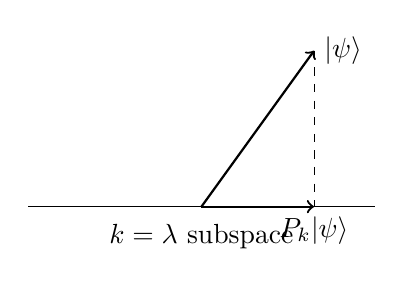
\begin{tikzpicture}[scale=1.1]
\draw (-2,0) -- (2,0);
\draw[->,thick] (0,0) -- (1.3,1.8) node[right] {$|\psi\rangle$};
\draw[dashed] (1.3,1.8) -- (1.3,0);
\draw[->,thick] (0,0) -- (1.3,0) node[below] {$P_k|\psi\rangle$};
\node at (0,-0.35) {$k=\lambda$ subspace};
\end{tikzpicture}
\caption{Projecting an arbitrary vector into the \(k=\lambda\) eigensubspace.}
\end{figure}

\begin{figure}[htbp]
\centering
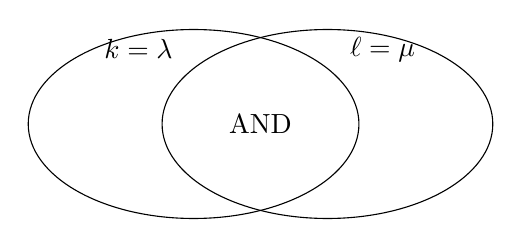
\begin{tikzpicture}[scale=1.0]
\draw (0,0) ellipse (2.1 and 1.2);
\draw (1.7,0) ellipse (2.1 and 1.2);
\node at (-0.7,0.95) {$k=\lambda$};
\node at (2.4,0.95) {$\ell=\mu$};
\node at (0.85,0) {AND};
\end{tikzpicture}
\caption{A reconstruction of the intersecting-subspace picture behind the AND statement for commuting projectors.}
\end{figure}

\begin{figure}[htbp]
\centering

\includegraphics[width=0.66\textwidth]{lecture_06_figure_08.png}
\caption{The board argument that commuting projectors select the simultaneous eigensubspace.}
\lectureframe{00:45:20}
\end{figure}

\begin{classroomqa}
\lecturetimestamp{00:44:42}
\audiencequestion{Is the simultaneous property the same as the intersection in classical logic?}
\lecturerresponse{Yes. For commuting projectors, \(P_kP_\ell\) projects onto the intersection of the two eigensubspaces. If the intersection contains only the zero vector, no nonzero state has both properties.}
\end{classroomqa}

For completeness, the projector onto the compatible OR subspace is
\begin{equation}
P_{k\lor\ell}=P_k+P_\ell-P_kP_\ell .
\end{equation}
When the alternatives are mutually exclusive, \(P_kP_\ell=0\) and this reduces to the sum \(P_k+P_\ell\). This subtraction is essential whenever the two subspaces overlap, because their intersection must not be counted twice.

Compatibility itself is then tied back to physical examples. In a two-spin system, any component \(\sigma_i\) of the first spin commutes with any component \(\tau_j\) of the second:
\begin{equation}
[\sigma_i,\tau_j]=0.
\end{equation}
By contrast, different components of the same spin do not commute:
\begin{equation}
[\sigma_1,\sigma_3]\neq 0.
\end{equation}
That is why one may measure one component of each of two separated spins, but not simultaneously measure two different components of the same spin.

\begin{classroomqa}
\lecturetimestamp{00:46:12}
\audiencequestion{What are concrete examples of compatible observables?}
\lecturerresponse{Any operator acting on the first spin commutes with every operator acting on the second, because they act on different tensor factors. Position components \(x,y,z\) are another compatible family. By contrast, two different components of the same spin, or position and its conjugate momentum, do not commute.}
\end{classroomqa}

\begin{classroomqa}
\lecturetimestamp{00:47:26}
\audiencequestion{Does a subsystem have to mean a different particle?}
\lecturerresponse{No. It means an independently specified set of degrees of freedom. Distinct particles give the simplest tensor factors, but different degrees of freedom of one particle can also be treated separately when their operator structure permits it.}
\end{classroomqa}

\begin{classroomqa}
\lecturetimestamp{00:48:37}
\audiencequestion{If so many operators on different subsystems commute, what is a simple incompatible pair?}
\lecturerresponse{Two components of the same spin provide the standard example: \(\sigma_1\) and \(\sigma_3\) do not commute, so no apparatus can assign both sharp values simultaneously. The nonzero matrix commutator is the algebraic test.}
\end{classroomqa}

Now Susskind revisits Bell's theorem. He does not redo last lecture's arithmetic. He rebuilds its logic in the new language. The classical inequality, in probabilistic form, is
\begin{equation}
P(A\wedge \neg B)+P(B\wedge \neg C)\ge P(A\wedge \neg C).
\end{equation}
This is a theorem of classical set logic, not of quantum mechanics. In the singlet state, spins are anti-aligned along any common axis, so a NOT statement for the first spin can be traded for the corresponding positive statement for the second. That lets one rewrite the inequality as a statement about joint properties of a two-spin system.

Suppressing identity operators on untouched factors, the single-property projectors appearing in the lecture are
\begin{equation}
\frac{1+\sigma_3}{2},\qquad
\frac{1+\frac{\tau_1+\tau_3}{\sqrt2}}{2},\qquad
\frac{1+\frac{\sigma_1+\sigma_3}{\sqrt2}}{2},\qquad
\frac{1+\tau_1}{2}.
\end{equation}
Therefore the three relevant joint projectors are
\begin{align}
\Pi_1 &= \frac{1+\sigma_3}{2}\,\frac{1+\frac{\tau_1+\tau_3}{\sqrt2}}{2}, \\
\Pi_2 &= \frac{1+\frac{\sigma_1+\sigma_3}{\sqrt2}}{2}\,\frac{1+\tau_1}{2}, \\
\Pi_3 &= \frac{1+\sigma_3}{2}\,\frac{1+\tau_1}{2}.
\end{align}

\begin{figure}[htbp]
\centering

\includegraphics[width=0.68\textwidth]{lecture_06_figure_09.png}
\caption{The three analyzer choices written as products of one-spin projectors.}
\lectureframe{01:01:45}
\end{figure}

The lecture speaks of the singlet in the familiar unnormalized blackboard form
\begin{equation}
|\Psi_{\mathrm{singlet}}\rangle \propto |ud\rangle-|du\rangle.
\end{equation}
The proportionality sign is enough here. What matters for the logic is the state itself and, in particular, the relative sign, not the overall normalization. Evaluating \(\langle \Pi_1\rangle+\langle \Pi_2\rangle\) against \(\langle \Pi_3\rangle\) in the singlet state yields the violation obtained in the previous lecture. The important conclusion is the one Susskind emphasizes verbally: quantum mechanics is not classical set theory in disguise.

\begin{classroomqa}
\lecturetimestamp{00:52:31}
\audiencequestion{If spin-up and spin-down are orthogonal, does the minus sign mean that one ket is the negative of the other?}
\lecturerresponse{No. \(|u\rangle\) and \(|d\rangle\) are distinct orthogonal vectors. A relative sign belongs to a superposition such as \(|ud\rangle-|du\rangle\) and can change its physical properties; only an overall sign multiplying the entire state is irrelevant.}
\end{classroomqa}

\begin{classroomqa}
\lecturetimestamp{00:53:06}
\audiencequestion{Is Bell's inequality violated for every quantum state and every choice of properties?}
\lecturerresponse{No. Many states and many choices of axes satisfy a particular Bell inequality. Violation depends on both the state and the selected observables. Varying the intermediate and final angles changes whether this test exposes the nonclassical correlations.}
\end{classroomqa}

\begin{classroomqa}
\lecturetimestamp{01:02:47}
\audiencequestion{What can be concluded when a particular state violates, or happens to satisfy, this Bell inequality?}
\lecturerresponse{A violation proves that the observed statistics cannot arise from the classical set logic used in the derivation. Satisfaction of one chosen inequality does not by itself make the state classical, because another choice of properties may reveal a violation.}
\end{classroomqa}

\section{Locality After Bell}

The projector calculation is not merely a symbolic game. Imagine repeatedly preparing correlated pairs in the singlet ground state, separating the two members, and dividing the identically prepared ensemble into three large groups. The first group measures the \(0^\circ\) and \(45^\circ\) settings, the second the \(45^\circ\) and \(90^\circ\) settings, and the third the \(0^\circ\) and \(90^\circ\) settings. Frequencies in the three groups estimate the three probabilities in the inequality.

\begin{classroomqa}
\lecturetimestamp{01:04:30}
\audiencequestion{What laboratory arrangement do the three Bell probabilities actually describe?}
\lecturerresponse{A source produces many identically prepared entangled pairs and sends the two members to separated analyzers. Split the pairs into three ensembles and use the corresponding pair of analyzer directions on each ensemble. Counting the joint outcomes estimates each probability. A charged particle and antiparticle could be separated by a field; practical Bell tests often use photons instead.}
\end{classroomqa}

\begin{classroomqa}
\lecturetimestamp{01:08:00}
\audiencequestion{The classical set proof used one population. How can three separately measured ensembles test it?}
\lecturerresponse{The inequality is a statement about probabilities as well as counts. If all three samples are drawn from the same preparation procedure, their relative frequencies estimate the three probability distributions of one common ensemble. Identical preparation is the indispensable assumption.}
\end{classroomqa}

That Bell recap leads straight into the physical unease still hanging over the room. If the correlations are real, why can they not be used to send a signal?

\begin{classroomqa}
\lecturetimestamp{01:09:41}
\audiencequestion{Why can the entangled correlations not be used to send a faster-than-light message?}
\lecturerresponse{Each wing separately still sees an uncontrollable random sequence. The correlation becomes visible only when the two records are compared through an ordinary classical channel. A decisive Bell test nevertheless arranges the choices and detections so that no light signal could pass between the wings in time, thereby excluding a local communication mechanism for producing the joint statistics.}
\end{classroomqa}

If enough time elapses for a light signal to travel between apparatuses, a correlation does not by itself contradict relativity; one might merely have discovered an unnoticed ordinary influence. The sharp experiment closes that escape route. In Bell's language, a hidden-variable account reproducing the correlations must be nonlocal, but nonlocal dependence is not the same thing as a controllable superluminal message.

\begin{classroomqa}
\lecturetimestamp{01:12:18}
\audiencequestion{Is angular momentum conservation essential to this argument?}
\lecturerresponse{No. Spin is a convenient two-state model, not a sacred ingredient. Any pair of two-level systems with the required entangled state and alternative measurement bases can display the same logical structure.}
\end{classroomqa}

This discussion does not close the lecture; it clears the ground for the next pivot. Bell has taught us that quantum mechanics is not classical logic, but the next question is different. What is a measurement, operationally and mathematically, and how does it enter the story of interference?

\section{Finite-State Two-Slit, Interference, and Measurement as Entanglement}

The lecture now changes model. Susskind turns to the two-slit experiment, but he immediately simplifies it into a finite-state problem so that the same vector-space technology can be used without bringing in the full machinery of continuum wave mechanics. He even says, in effect, that this is still the two-slit experiment, only stripped down to a small set of basis states.

There is a source state \(|0\rangle\), two slit states \(|1\rangle\) and \(|-1\rangle\), and a set of screen states \(|n\rangle\). These \(|n\rangle\) are orthonormal because distinct screen positions are distinct configurations. The lecture explicitly chooses not to track normalization carefully here. Unitarity is postponed. What matters at this stage is linearity.

\begin{figure}[htbp]
\centering
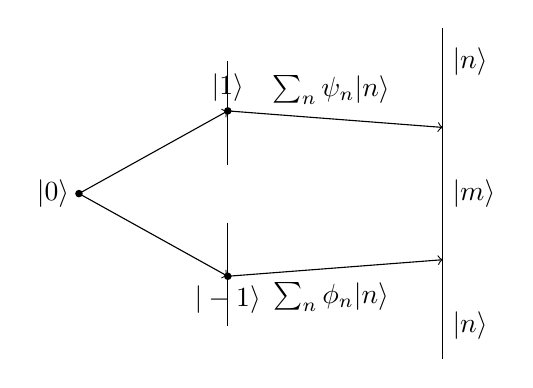
\begin{tikzpicture}[scale=1.05]
\fill (0,0) circle (1.3pt);
\node[left] at (0,0) {$|0\rangle$};

\draw (1.8,1.6) -- (1.8,0.35);
\draw (1.8,-0.35) -- (1.8,-1.6);
\fill (1.8,1) circle (1.3pt);
\fill (1.8,-1) circle (1.3pt);
\node[above] at (1.8,1) {$|1\rangle$};
\node[below] at (1.8,-1) {$|-1\rangle$};

\draw (4.4,2.0) -- (4.4,-2.0);
\node[right] at (4.4,1.6) {$|n\rangle$};
\node[right] at (4.4,0.0) {$|m\rangle$};
\node[right] at (4.4,-1.6) {$|n\rangle$};

\draw[->] (0,0) -- (1.8,1);
\draw[->] (0,0) -- (1.8,-1);
\draw[->] (1.8,1) -- (4.4,0.8);
\draw[->] (1.8,-1) -- (4.4,-0.8);

\node at (3.05,1.25) {$\sum_n \psi_n |n\rangle$};
\node at (3.05,-1.25) {$\sum_n \phi_n |n\rangle$};
\end{tikzpicture}
\caption{A finite-state version of the two-slit experiment: the source state \(|0\rangle\), the two slit states \(|1\rangle\) and \(|-1\rangle\), and the screen basis \(|n\rangle\).}
\end{figure}

\begin{figure}[htbp]
\centering

\includegraphics[width=0.68\textwidth]{lecture_06_figure_10.png}
\caption{The finite position lattice beside the linear evolution rule \(A\to A'\), \(B\to B'\).}
\lectureframe{01:18:00}
\end{figure}

By symmetry the source evolves to an equal-amplitude superposition of the two slit states:
\begin{equation}
|0\rangle \longrightarrow |1\rangle+|-1\rangle.
\end{equation}
Now let the upper slit state evolve to
\begin{equation}
|1\rangle \longrightarrow \sum_n \psi_n |n\rangle,
\end{equation}
and the lower slit state to
\begin{equation}
|-1\rangle \longrightarrow \sum_n \phi_n |n\rangle.
\end{equation}
The arrows here mean time evolution, not equality of states at the same instant. By linearity,
\begin{equation}
|1\rangle+|-1\rangle \longrightarrow \sum_n (\psi_n+\phi_n)|n\rangle.
\end{equation}
That is the key rule. Amplitudes add before probabilities are formed.

\begin{classroomqa}
\lecturetimestamp{01:21:59}
\audiencequestion{How can the slit state \(|1\rangle\) turn into states also labelled by integers \(n\)? Are these kets at the same place and time?}
\lecturerresponse{The labels refer to different time slices. \(|1\rangle\) denotes the electron at the upper slit, whereas the \(|n\rangle\) on the right denote possible later positions on the screen. The arrow is time evolution, not an equality between simultaneous configurations.}
\end{classroomqa}

\begin{classroomqa}
\lecturetimestamp{01:25:30}
\audiencequestion{Should the amplitudes be normalized, and do they carry physical units?}
\lecturerresponse{A complete evolution must preserve total probability; that is unitarity. Here the common normalization is suppressed because only the addition and cancellation of path amplitudes matter. Any scale factors can be restored when the state is normalized.}
\end{classroomqa}

The probability of arrival at the screen site \(m\) is therefore
\begin{align}
P_m &= |\psi_m+\phi_m|^2 \\
    &= |\psi_m|^2 + |\phi_m|^2 + \psi_m^*\phi_m + \phi_m^*\psi_m.
\end{align}
The first two terms are what classical reasoning would have produced. The last two are the interference terms.

\begin{figure}[htbp]
\centering

\includegraphics[width=0.68\textwidth]{lecture_06_figure_11.png}
\caption{The screen amplitude and its four-term probability expansion on the board.}
\lectureframe{01:29:20}
\end{figure}

At the symmetric point on the screen, call it \(m=0\), symmetry suggests \(\psi_0=\phi_0\). Then
\begin{equation}
P_0 = |\psi_0+\phi_0|^2 = |2\psi_0|^2 = 4|\psi_0|^2.
\end{equation}
Both slits open produce four times the one-slit probability at that point, not twice. This is constructive interference.

Now insert a phase shift so that \(\phi_0=-\psi_0\). Then
\begin{equation}
P_0 = |\psi_0-\psi_0|^2 = 0.
\end{equation}
Each slit by itself permits arrival at that point, but opening both together can make arrival there impossible. This is destructive interference. Susskind explicitly dwells on how odd this is: for his money it is as strange as Bell.

\begin{classroomqa}
\lecturetimestamp{01:33:14}
\audiencequestion{What if the phase shifter or slit choice is changed only after the electron is already in flight? Does the other slit need time to learn about it?}
\lecturerresponse{The answer depends on the precise spacetime arrangement and on whether the electron encounters the altered part of the apparatus. Quantum mechanics evolves the state through the actual setup; probabilities still come from adding the applicable amplitudes. A delayed-choice proposal must be specified sharply before locality claims can be assessed.}
\end{classroomqa}

Now we introduce the apparatus. There is one additional two-state system, a spin initially in the state \(|d\rangle\). If the electron goes through the upper slit, it flips that spin to \(|u\rangle\). If it goes through the lower slit, it leaves it unchanged. The initial composite state is \(|0,d\rangle\), and the first update rule becomes
\begin{equation}
|0,d\rangle \longrightarrow |1,u\rangle + |-1,d\rangle.
\end{equation}
That one line is the whole meaning of measurement in the lecture. The position of the electron has become entangled with the record stored in the apparatus.

\begin{figure}[htbp]
\centering

\includegraphics[width=0.66\textwidth]{lecture_06_figure_12.png}
\caption{The detector spin correlates its up and down records with the two slit alternatives.}
\lectureframe{01:44:10}
\end{figure}

\begin{classroomqa}
\lecturetimestamp{01:40:20}
\audiencequestion{Must there be a detector at both slits?}
\lecturerresponse{One reliable detector is enough. If it records passage through the upper slit, an unchanged record identifies the lower alternative, provided every transmitted electron must pass through one of the two openings. A second detector is possible but adds another subsystem without changing the principle.}
\end{classroomqa}

\begin{classroomqa}
\lecturetimestamp{01:40:51}
\audiencequestion{Why not say that the electron passes through both slits?}
\lecturerresponse{Without a path record, the state is a coherent superposition and no retrospective path fact is available. With a complete which-path measurement, the apparatus records one alternative or the other on each run. What persists through both alternatives is the state amplitude, not two separately observed electron trajectories.}
\end{classroomqa}

\begin{figure}[htbp]
\centering
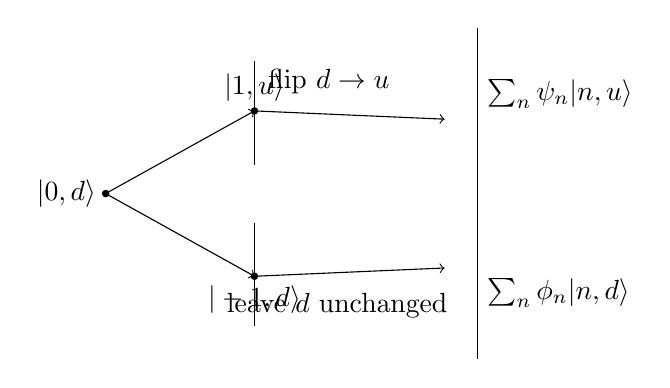
\begin{tikzpicture}[scale=1.05]
\fill (0,0) circle (1.3pt);
\node[left] at (0,0) {$|0,d\rangle$};

\draw (1.8,1.6) -- (1.8,0.35);
\draw (1.8,-0.35) -- (1.8,-1.6);
\fill (1.8,1) circle (1.3pt);
\fill (1.8,-1) circle (1.3pt);
\node[above] at (1.8,1) {$|1,u\rangle$};
\node[below] at (1.8,-1) {$|-1,d\rangle$};

\draw (4.5,2.0) -- (4.5,-2.0);
\node[right] at (4.5,1.2) {$\sum_n \psi_n |n,u\rangle$};
\node[right] at (4.5,-1.2) {$\sum_n \phi_n |n,d\rangle$};

\draw[->] (0,0) -- (1.8,1);
\draw[->] (0,0) -- (1.8,-1);
\draw[->] (1.8,1) -- (4.1,0.9);
\draw[->] (1.8,-1) -- (4.1,-0.9);

\node at (2.7,1.35) {flip \(d\to u\)};
\node at (2.8,-1.35) {leave \(d\) unchanged};
\end{tikzpicture}
\caption{Measurement as entanglement with a detector spin. The upper path flips the apparatus spin; the lower path leaves it untouched.}
\end{figure}

Assume, as the lecture does, that nothing further happens to the spin during the journey to the screen. Then
\begin{align}
|1,u\rangle &\longrightarrow \sum_n \psi_n |n,u\rangle, \\
|-1,d\rangle &\longrightarrow \sum_n \phi_n |n,d\rangle.
\end{align}
Therefore the final state with both slits open is
\begin{equation}
|\Psi_{\mathrm{final}}\rangle
  = \sum_n \psi_n |n,u\rangle + \sum_n \phi_n |n,d\rangle.
\end{equation}
This is not a superposition of states of one electron alone. It is an entangled state of electron and apparatus.

\begin{figure}[htbp]
\centering

\includegraphics[width=0.68\textwidth]{lecture_06_figure_13.png}
\caption{The two path amplitudes reach the screen carrying orthogonal apparatus records.}
\lectureframe{01:47:35}
\end{figure}

The cleanest way to compute the arrival probability at the site \(m\) is to use the projector onto that site on the electron subsystem:
\begin{equation}
\Pi_m = |m\rangle\langle m|\otimes I_{\mathrm{spin}}.
\end{equation}
Applying \(\Pi_m\) to the final state gives
\begin{equation}
\Pi_m |\Psi_{\mathrm{final}}\rangle
= |m\rangle\bigl(\psi_m|u\rangle+\phi_m|d\rangle\bigr).
\end{equation}
So the probability of arrival at \(m\) is
\begin{align}
P_m
  &= \langle \Psi_{\mathrm{final}}|\Pi_m|\Psi_{\mathrm{final}}\rangle \\
  &= \bigl(\psi_m^*\langle u|+\phi_m^*\langle d|\bigr)
     \bigl(\psi_m|u\rangle+\phi_m|d\rangle\bigr) \\
  &= |\psi_m|^2 + |\phi_m|^2
     + \psi_m^*\phi_m\langle u|d\rangle
     + \phi_m^*\psi_m\langle d|u\rangle.
\end{align}
But the record states are orthogonal:
\begin{equation}
\langle u|d\rangle=0.
\end{equation}
Hence the cross terms vanish:
\begin{equation}
P_m = |\psi_m|^2 + |\phi_m|^2.
\end{equation}
That is the lecture's mathematical punchline. Once which-path information is recorded, interference disappears and probabilities add in the classical way.

\begin{classroomqa}
\lecturetimestamp{01:49:09}
\audiencequestion{What is the difference between the superposition \(|1\rangle+|-1\rangle\) and the state \(|1,u\rangle+|-1,d\rangle\)?}
\lecturerresponse{The first concerns one system in a linear combination of two positions; there is nothing else with which it could be entangled. The second concerns two systems and correlates path with detector spin. Reading the spin then reveals information about the path.}
\end{classroomqa}

\section{Environmental Records and Partial Measurement}

A deliberately built detector is not the only recorder. An atom near a slit, residual gas, a thermal surface, or any other degree of freedom can become correlated with the path. If its final states are \(|E_1\rangle\) and \(|E_2\rangle\), the path state has the form
\begin{equation}
|\Psi\rangle
=\sum_n\left(\psi_n|n\rangle|E_1\rangle
+\phi_n|n\rangle|E_2\rangle\right).
\end{equation}
The interference terms are now multiplied by the overlap \(\langle E_1|E_2\rangle\). Orthogonal records make the paths perfectly distinguishable and erase interference completely. Identical records leave \(\langle E_1|E_2\rangle=1\) and preserve it. Intermediate overlap gives partial visibility.

\begin{figure}[htbp]
\centering

\includegraphics[width=0.68\textwidth]{lecture_06_figure_14.png}
\caption{Overlapping and separated environmental wave packets illustrate partial and complete path records.}
\lectureframe{01:53:40}
\end{figure}

\begin{classroomqa}
\lecturetimestamp{01:50:48}
\audiencequestion{Would an ordinary atom near the slit become entangled with the passing electron even if nobody deliberately observes it?}
\lecturerresponse{Yes. Knowledge is not the operative verb; physical correlation is. If the atom or surrounding gas is disturbed enough that its later state distinguishes the path, it records which-way information and suppresses interference. This is why such experiments require isolation, low temperatures, and often weakly interacting particles such as photons.}
\end{classroomqa}

Cooling places environmental degrees of freedom near their ground states and reduces accidental records. An energy gap helps as well: if the incident particle cannot supply the minimum excitation energy, the environment may be unable to retain path information. Conversely, charged particles can disturb nearby matter through their electric fields, making electron interference especially demanding.

\begin{classroomqa}
\lecturetimestamp{01:54:49}
\audiencequestion{Can an interference pattern really be obtained with single electrons?}
\lecturerresponse{Each electron makes only one localized hit. Send the particles through one at a time, with enough separation that they cannot interact, and collect many repetitions. The accumulated frequency distribution displays the interference pattern; one event alone is only a blip.}
\end{classroomqa}

\begin{classroomqa}
\lecturetimestamp{01:55:59}
\audiencequestion{Does measurement destroy entanglement or create it?}
\lecturerresponse{The which-path interaction creates entanglement between system and apparatus, and that entanglement destroys interference between the alternatives. A later measurement can correlate the apparatus with yet another system and may condition the remaining state, so one must always say which two subsystems and which interference are being discussed.}
\end{classroomqa}

\begin{classroomqa}
\lecturetimestamp{01:57:44}
\audiencequestion{Can the interaction be weakened so that the apparatus obtains only partial path information?}
\lecturerresponse{Yes. A weak interaction may flip the detector only with some amplitude, leaving nonorthogonal record states. Then the paths are only partly distinguishable and the interference is only partly reduced. Stronger measurement means greater distinguishability, stronger entanglement with the record, and lower fringe visibility.}
\end{classroomqa}

The collapse relevant here is therefore concrete: it is the loss of the cross terms when path information has been deposited in another system. With no record, amplitudes add. With perfectly distinguishable records, their inner products vanish and probabilities add. Between those extremes, measurement strength and interference visibility vary continuously.
